\documentclass[a4paper, 12pt]{book}
% preamble.tex

\usepackage[utf8]{inputenc}
\usepackage[T1]{fontenc}
\usepackage[english]{babel} % Ho cambiato in italian, supponendo che la maggior parte del testo sia in italiano
\usepackage{amsmath}
\usepackage{amssymb}
\usepackage{graphicx}
\usepackage{hyperref}
\usepackage{geometry}
\usepackage{fontspec} % Utile per Xetex/LuaLaTeX ma mantenuto
\usepackage{booktabs}
\usepackage{amsthm}
\usepackage{enumitem}
\usepackage{caption}
\usepackage{thmtools}
\usepackage{standalone} % Già presente nel tuo elenco
\usepackage{tkz-euclide}
\usepackage{graphicx}
\usepackage[T1]{fontenc}
\usepackage{wesa}

% --- PACCHETTI AGGIUNTI PER LA FORMATTAZIONE ---
\usepackage{parskip}  % Aggiunge spazio tra i paragrafi (stile "blocco")
\usepackage{fancyhdr} % Per intestazioni e piè di pagina personalizzati

% --- IMPOSTAZIONI GEOMETRIA E FONT ---
\geometry{a4paper, margin=1in}

% Configura lo stile 'plain' (usato da \maketitle e \tableofcontents)
% per essere coerente con il piè di pagina
\fancypagestyle{plain}{
    \fancyhf{} % Pulisce
    \cfoot{\thepage} % Mette solo il numero di pagina
    \renewcommand{\headrulewidth}{0pt} % Niente linea su queste pagine
}

% Configurazione Header/Footer per le altre pagine
\pagestyle{fancy}
\fancyhead{} % Pulisce l'intestazione
\fancyfoot{} % Pulisce il piè di pagina
\fancyhead[L]{\nouppercase{\rightmark}} % Nome Sezione a sinistra (o Chapter)
\fancyhead[R]{\nouppercase{\leftmark}}  % Nome Capitolo a destra (o Sezione)
\fancyfoot[C]{\thepage} % Numero di pagina al centro
\renewcommand{\headrulewidth}{0.4pt}
\renewcommand{\footrulewidth}{0pt}


% --- DEFINIZIONI TEOREMI ---
% (Questa parte è cruciale per la tua struttura)
\newtheoremstyle{mythmstyle}%
    {}%
    {}%
    {\itshape}%
    {}%
    {\bfseries}%
    {}%
    { }%
    {\thmname{#1}\thmnumber{ #2}%
    \thmnote{: #3\addcontentsline{toc}{subsubsection}{{\itshape#1}: #3}}. }

% 2. Imposta questo stile come quello ATTUALE
\theoremstyle{mythmstyle}

\newtheorem{theorem}{Th}[section]
\newtheorem{definition}{Def}[section]
\newtheorem{proposition}{Prop}[section]
\newtheorem{corollary}{Cor}[section]
\newtheorem{algorithm}{Alg}[section]
\newtheorem{lemma}{Lemma}[section]
\newtheorem*{remark}{Rem}

% Definizioni utili per il Main file
\newcommand{\inputlesson}[1]{\clearpage\input{#1}\clearpage} % Comando per input lezione
\usepackage[x11names, table]{xcolor}
\usepackage{tikz}
\usetikzlibrary{shapes,fit}
\usetikzlibrary{positioning, arrows.meta, shapes.geometric}
\usepackage{amsmath} % Required for align environment
\usepackage{colortbl}
\usetikzlibrary{shapes, arrows, positioning}



\begin{document}
\setcounter{chapter}{4}
\chapter[ ]{Lesson 25-11-2025}

% Pacchetti necessari da assicurarsi di avere nel preambolo per compilare questo snippet:
% \usepackage{tikz}

% \usepackage{xcolor}


\section{Linear channel equalization}

Ref: \textit{A signal processing perspective} (pp. 57-130), p. 31.

\subsection{Introduction: super basic block scheme}

It's a pretty old topic.\\
We have a transmitter, then a channel, then a noise which is added \textbf{before} anything else.

\vspace{1em}
\begin{center}
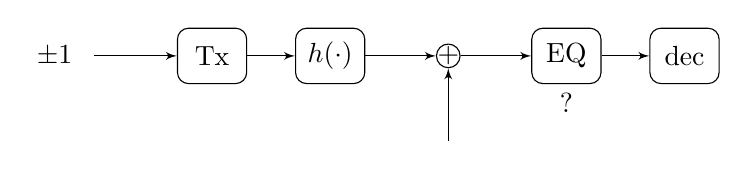
\begin{tikzpicture}[auto, node distance=1.5cm, >=latex']
    % Stili
    \tikzstyle{block} = [draw, rectangle, rounded corners, minimum height=2em, minimum width=2.5em]
    \tikzstyle{sum} = [draw, circle, inner sep=0pt, minimum size=3mm]
    \tikzstyle{input} = [coordinate]
    \tikzstyle{output} = [coordinate]

    % Nodi
    \node [input] (in) {};
    \node [left of=in, node distance=0.5cm] (lbl) {$\pm 1$};
    \node [block, right of=in] (tx) {Tx};
    \node [block, right of=tx] (h) {$h(\cdot)$};
    \node [sum, right of=h] (sum) {};
    % Disegna la croce nel nodo somma
    \node at (sum) {+};
    \node [block, right of=sum] (eq) {EQ};
    \node [block, right of=eq] (dec) {dec};
    \node [below of=sum, node distance=1.2cm] (noise) {};

    % Collegamenti
    \draw [->] (in) -- (tx);
    \draw [->] (tx) -- (h);
    \draw [->] (h) -- (sum);
    \draw [->] (sum) -- (eq);
    \draw [->] (eq) -- (dec);
    \draw [->] (noise) -- (sum);

    % Annotazione EQ
    \node [below of=eq, node distance=0.6cm] {?};
\end{tikzpicture}
\end{center}
\vspace{1em}

% Definizione colore locale se non presente (rimuovi se definito nel preambolo)

% Primo Riquadro Verde
\noindent
\colorbox{obsidianGreen}{%
    \begin{minipage}{\dimexpr\linewidth-2\fboxsep}
    \setlength{\parskip}{0.5em}
    About magnetic writing; we're writing on a tape, which is noisy; we need to encode before writing.\\
    Fractional sampling: we're sampling at multiples of the Nyquist rate; it's used in order to synchronize.
    \end{minipage}%
}

\vspace{0.5em}

% Secondo Riquadro Verde
\noindent
\colorbox{obsidianGreen}{%
    \begin{minipage}{\dimexpr\linewidth-2\fboxsep}
    We don't need to have $\pm 1$, it can just be whichever input.
    \end{minipage}%
}

\subsection{Feedback equalizer}

If we have that at a certain time the receive signal is
\begin{align}
    y(0) = h(0)x(0) + h(1)x(-1) \,,
\end{align}
how do we equalize this?

First of all, we'd need to estimate the channel: this means trying to understand the values of $h(0), h(1)$.\\
If we suppose we estimated $x(-1)$ as $\hat{x}(-1)$, what we do is implement a feedback equalizer: we'll look at

\begin{align}
    \frac{y(0) - h(1)\hat{x}(-1)}{h(0)}
\end{align}

which will get us $x(0)$.

We can estimate $\hat{x}(-1)$ since we generally have packets: we know the first symbols, thus we can \textit{bootstrap} this machine.

This is the feedback equalizer:
\begin{center}
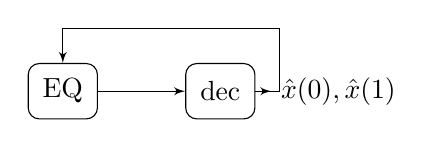
\begin{tikzpicture}[auto, node distance=1.5cm, >=latex']
    % Stili
    \tikzstyle{block} = [draw, rectangle, rounded corners, minimum height=2em, minimum width=2.5em]
    \tikzstyle{input} = [coordinate]
    \tikzstyle{output} = [coordinate]

    % Nodi
    \node [block] (eq) {EQ};
    \node [block, right of=eq, node distance=2cm] (dec) {dec};
    \node [right of=dec, node distance=1.5cm] (out) {$\hat{x}(0), \hat{x}(1)$};

    % Collegamenti
    \draw [->] (eq) -- (dec);
    \draw [->] (dec) -- (out);
    
    % Feedback loop
    \draw [->] (dec.east) -- ++(0.3,0) -- ++(0,0.8) -| (eq.north);

\end{tikzpicture}
\end{center}

It's also true that if we fail in decoding a symbol, this could be catastrophic: this would lead to a chain of errors.\\
We need to play with this type of equalization very carefully.

\subsection[Linear zero forcing equalization]{Linear zero forcing equalization (for both SISO and MIMO; only in the $z$ domain); example 2.17}

We'll see just something, but if we want to know more we can look at other books.

What we do is that we go in the $z$ domain (see \textcolor{green}{z transform}); when we have a sequence, such as $h[0], h[1], h[2], \dots$, we'll write it as
\begin{align}
    \mathbf{h}(z) = h_0 + h_1 z^{-1} + h_2 z^{-2} \,.
\end{align}

\vspace{0.5em}
\noindent
\colorbox{obsidianGreen}{%
    \begin{minipage}{\dimexpr\linewidth-2\fboxsep}
    We can revise this by looking at signals and systems.\\
    A delay of $n$ in the time domain corresponds to a multiplication with $z^{-n}$ in the $z$ domain.
    \end{minipage}%
}
\vspace{0.5em}

We want to find an equalizer $w^*(z)$ such that the combination with $\mathsf{h}(z)$ is just a delay (this is the Heaviside condition):

\begin{align}
    w^*(z)\sqrt{G}h(z) = z^{-\Delta} \,. \tag{2.124}
\end{align}

The delay is a degree of freedom which can be used when designing.

We however can see that $w^*(z)$ \textbf{might not exist or it might be unstable}.

According to the zero-forcing criteria, we'd have
\begin{align}
    w^*(z) = \frac{1}{\mathbf{h}(z)} \cdot \frac{z^{-\Delta}}{\sqrt{G}} \,;
\end{align}
we first of all ask ourselves: \textbf{is this stable?} If it's not stable, the noise coming in might make our system explode!\\
The system is BIBO if the root of the polynomial $w^*(z)$ is inside the unit circle. The noise, even if bounded, might not be bounded after the system.\\
This is the problem of the zero forcing; the zero forcing means that we want to just have a single delay; point is that we might have just a delay but with a non-stable filter.

We then ask ourselves: \textbf{is the response $w^*(z)$ finite or infinite?} $\rightarrow$ most of the time is \textbf{infinite}

\begin{center}
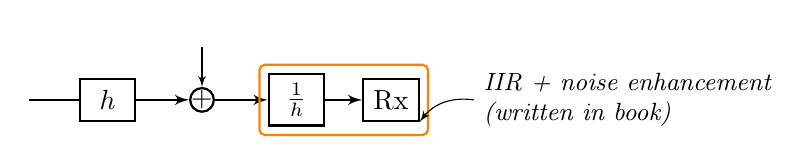
\begin{tikzpicture}[auto, node distance=1.5cm, >=latex']
    % Definisco gli stili mancanti
    \tikzstyle{block} = [draw, rectangle, minimum height=1.5em, minimum width=2em, thick]
    \tikzstyle{sum} = [draw, circle, inner sep=0pt, minimum size=3mm, thick]
    \tikzstyle{input} = [coordinate] % <--- Mancava questa definizione
    
    % Nodi
    \node [input] (in) {};
    \node [block, right of=in, node distance=1cm] (h) {$h$};
    \node [sum, right of=h, node distance=1.2cm] (sum) {};
    \node at (sum) {+};
    \node [block, right of=sum, node distance=1.2cm] (invh) {$\frac{1}{h}$};
    \node [block, right of=invh, node distance=1.2cm] (rx) {Rx};
    
    % Noise input to sum
    \node [above of=sum, node distance=0.8cm] (noise) {};
    \draw [->] (noise) -- (sum);

    % Collegamenti
    \draw [thick] (in) -- (h);
    \draw [->, thick] (h) -- (sum);
    \draw [->, thick] (sum) -- (invh);
    \draw [->, thick] (invh) -- (rx);

    % Riquadro arancione intorno a 1/h e Rx
    % Nota: Richiede il pacchetto \usetikzlibrary{fit} nel preambolo
    \node[draw=orange, thick, fit=(invh) (rx), inner sep=3pt, rounded corners=2pt] {};

    % Nota scritta a mano
    \node [right of=rx, node distance=3cm, align=left, font=\small\itshape] (note) {IIR + noise enhancement\\(written in book)};
    \draw [->, bend right, thin] (note.west) to (rx.south east);

\end{tikzpicture}
\end{center}

We'll then look at the zero forcing \textbf{in the MIMO case}. The interesting result is that here for many types of FIR multivariate channel we have FIR zero forcing equalizers, given that we're under certain conditions.

Let's say that the Z-transform of $H[0], \dots, H[L]$ is
\begin{align}
    \mathbf{H}(z) = \sum_{\ell=0}^{L} \mathbf{H}[\ell]z^{-\ell} \,; \tag{2.129}
\end{align}

this implies that the channel will become a polynomial and \textbf{we'll look for an equalizer} $\mathbf{W}^*(z)$ such that

\begin{align}
    \mathbf{W}^*(z)\sqrt{G}\mathbf{H}(z) = \mathbf{D}(z) \,, \tag{2.130}
\end{align}

where

\begin{itemize}
    \item $\mathbf{D}(z)$ is a diagonal matrix containing possibly different delay terms in the form of $z^{-\Delta}$.
\end{itemize}

% Inserimento diagramma manoscritto ricostruito qui, pertinente ai ritardi
\begin{center}
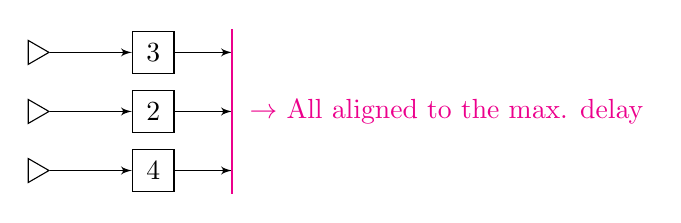
\begin{tikzpicture}[>=latex']
    \tikzstyle{buffer} = [draw, regular polygon, regular polygon sides=3, shape border rotate=-90, inner sep=1pt, fill=white, minimum height=1em]
    \tikzstyle{delay} = [draw, rectangle, minimum size=1.5em, fill=white]
    
    % Linea 1
    \node[buffer] (b1) at (0, 1.5) {};
    \node[delay] (d1) at (1.5, 1.5) {3};
    \draw[->] (b1) -- (d1);
    \draw[->] (d1) -- (2.5, 1.5);
    
    % Linea 2
    \node[buffer] (b2) at (0, 0.75) {};
    \node[delay] (d2) at (1.5, 0.75) {2};
    \draw[->] (b2) -- (d2);
    \draw[->] (d2) -- (2.5, 0.75);
    
    % Linea 3
    \node[buffer] (b3) at (0, 0) {};
    \node[delay] (d3) at (1.5, 0) {4};
    \draw[->] (b3) -- (d3);
    \draw[->] (d3) -- (2.5, 0);
    
    % Linea verticale di allineamento e nota rosa
    \draw[magenta, thick] (2.5, 1.8) -- (2.5, -0.3);
    \node[magenta, anchor=west] at (2.6, 0.75) {$\rightarrow$ All aligned to the max. delay};

    % Decorazione stile griglia quaderno (opzionale, per contesto)
    %\draw[step=0.25cm,gray!20,very thin] (-1,-0.5) grid (6,2);
\end{tikzpicture}
\end{center}

One thing which should be noted is that \textbf{we need to have that a left inverse exists for $\mathbf{H}$ in order for the equalizer to exist}; if we cannot have a left inverse (for various reasons, such as $\mathbf{H}$ not being full-rank), then \textbf{we won't have an equalizer}.\\
One condition which is considered already from this moment is that (quoting from the book):

\vspace{1em}
% Callout Blu
\noindent
\colorbox{obsidianBlue}{%
    \begin{minipage}{\dimexpr\linewidth-2\fboxsep}
    \vspace{0.3em}
    \textcolor{obsidianTextBlue}{\textbf{\faPen\ Existence of a left FIR inverse}}
    
    A MIMO transfer function $\mathbf{H}(z)$ has a left FIR inverse iff $\mathbf{H}(z)$ has full column rank for every complex $z \neq 0$.
    \vspace{0.3em}
    \end{minipage}%
}
\vspace{1em}

Some other conditions will be tackled later, but just as an anticipation, they'll result in saying that the ZF equalizer exists only if

\begin{align}
    N_t(L_{eq} + L + 1) \leq N_r(L_{eq} + 1) \tag{2.146+}
\end{align}

\vspace{1em}
% Callout Viola
\noindent
\colorbox{obsidianPurple}{%
    \begin{minipage}{\dimexpr\linewidth-2\fboxsep}
    \vspace{0.3em}
    \textcolor{obsidianTextPurple}{\textbf{\faBook\ What was $H[\ell]$ again?}}
    
    We know that $\mathbf{H}[\ell]$ is a matrix such that
    \[ [\boldsymbol{H}[\ell]]_{i,j} = h_{i,j}[\ell] \]
    is the channel's response between receiving antenna $i$ and transmitting antenna $j$.\\
    From this, it will follow that
    \[ [\mathbf{H}(z)]_{i,j} = \mathcal{Z}[h_{i,j}[\cdot]] \, z \,. \]
    \vspace{0.1em}
    \end{minipage}%
}
\vspace{1em}

\vspace{1em}
% Callout Giallo
\noindent
\colorbox{obsidianYellow}{%
    \begin{minipage}{\dimexpr\linewidth-2\fboxsep}
    \vspace{0.3em}
    \textcolor{obsidianTextYellow}{\small \faQuoteLeft\ \textit{A signal processing perspective} (pp. 57-130), p. 33}
    
    As in the SISO case, it is in practice desirable to restrict the focus to FIR equalizers, meaning that each entry of $\mathbf{w}(z)$ corresponds to an FIR filter of order $L_{eq}$. Do exact left inverses of $\mathbf{H}(z)$ exist? Yes, as it turns out. More precisely, the answer is found in what is called \textbf{perfect recoverability}.
    \vspace{0.3em}
    \end{minipage}%
}
\vspace{1em}

So, if the \textit{perfect recoverability} holds, we'll be sure to find left inverses of the $\mathbf{H}$ matrix; we need the left inverse since it will be used when we'll determine the ZF equalizer.

% --- PAGINA 1 ---

Here in \textbf{MIMO FIR filters may exist!} Before, in SISO, \textbf{they might have not!}

About matrices: until now we saw that the inverse of whichever matrix $\boldsymbol{A}$ is such that $\boldsymbol{A}\boldsymbol{A}^{-1} = \boldsymbol{I}$ and $\boldsymbol{A}^{-1}\boldsymbol{A} = \boldsymbol{I}$; this only holds if it's square; generally, the left and right inverses are different.

\vspace{1em}

% Riquadro Viola Piccolo (About this paragraph)
\noindent
\begin{tikzpicture}
\node [draw=obsidianBorderPurple, fill=obsidianPurple, inner sep=5pt, rounded corners, text width=\dimexpr\linewidth-12pt\relax] {
    \textcolor{obsidianTextPurple}{\textbf{\faExclamationCircle\ About this paragraph}}\\
    \footnotesize
    The notation we wrote here just gives an idea; everything will be treated in the time domain.
};
\end{tikzpicture}

\vspace{1em}

% Riquadro Esempio 2.17 - PARTE 1
\noindent
\begin{tikzpicture}
\node [draw=obsidianBorderPurple, inner sep=10pt, rounded corners, text width=\dimexpr\linewidth-22pt\relax] (box1){%
    \begin{minipage}{\linewidth}
    \textcolor{obsidianTextPurple}{\textbf{\faList\ Example 2.17}}
    \vspace{0.5em}
    
    {\footnotesize For $N_t=1$ and $N_r=2$, find the conditions on $\mathbf{H}(z)$ such that FIR ZF equalizers exist.}
    \vspace{1em}

    If we have 1 transmit antenna and 2 receive antennas; in general we might transmit to both antennas:

    \begin{center}
    \begin{tikzpicture}[>=latex', scale=0.9]
        % Antenna TX
        \draw[thick] (0,0) -- (0,-0.5);
        \draw[thick] (0,0) -- (-0.2,0.4);
        \draw[thick] (0,0) -- (0.2,0.4);
        \node at (0,-0.8) {Tx};

        % Antenne RX
        \begin{scope}[xshift=4cm, yshift=0.8cm]
            \draw[thick] (0,0) -- (0,-0.5);
            \draw[thick] (0,0) -- (-0.2,0.4);
            \draw[thick] (0,0) -- (0.2,0.4);
            \node at (0.5,-0.2) {Rx1};
            \node at (-0.5,0) (rx1node) {};
        \end{scope}

        \begin{scope}[xshift=4cm, yshift=-0.8cm]
            \draw[thick] (0,0) -- (0,-0.5);
            \draw[thick] (0,0) -- (-0.2,0.4);
            \draw[thick] (0,0) -- (0.2,0.4);
            \node at (0.5,-0.2) {Rx2};
            \node at (-0.5,0) (rx2node) {};
        \end{scope}

        % Frecce canale
        \draw[->] (0.2, 0) -- (3.5, 0.6);
        \draw[->] (0.2, 0) -- (3.5, -0.6);
        
        % Simbolo Psi
        \node at (1.5, 0) {$\Psi$}; 
    \end{tikzpicture}
    \end{center}

    % Box verde interno
    \noindent
    \colorbox{obsidianGreen}{%
        \begin{minipage}{\dimexpr\linewidth-2\fboxsep}
        \textcolor{gray}{\vrule width 2pt} \hspace{0.5em} Digital always includes a delay!
        \end{minipage}%
    }
    \vspace{1em}

    We then need to decide what to do; \textbf{we might think about selecting the stronger signal}; one might have a reflection and such; this is called \textbf{antenna selection}.\\
    \textbf{It's easy to measure the amplitude of a signal, but we can't know whether the signal is clean}.\\
    Someone came up with something called \textbf{MRC (Max Ratio Combining): we weight each signal with the complex conjugate}; this allows us \textbf{to have the best SNR}. This is still done, even with analog transmissions.

    What we have is that we want to satisfy
    \begin{align}
        [\mathbf{W}(z)]_0^* \sqrt{G} \, [\mathbf{H}(z)]_0 + [\mathbf{W}(z)]_1^* \sqrt{G} \, [\mathbf{H}(z)]_1 = z^{-\Delta} \,.
    \end{align}

    $\mathbf{H}(z)$ is a column vector:
    
    \vspace{1em}
    \begin{center}
    $\downarrow$ \textit{read example (continued on next page)}
    \end{center}
    \end{minipage}
};
\end{tikzpicture}

\vfill
\clearpage 

% --- PAGINA 2 ---

% Riquadro Esempio 2.17 - PARTE 2
\noindent
\begin{tikzpicture}
\node [draw=obsidianBorderPurple, inner sep=10pt, rounded corners, text width=\dimexpr\linewidth-22pt\relax] (box2){%
    \begin{minipage}{\linewidth}
    \textcolor{obsidianTextPurple}{\textbf{\faList\ Example 2.17 (continued)}}
    \vspace{0.5em}

    \begin{center}
    \begin{tikzpicture}[auto, >=latex', node distance=2.5cm]
        \node[circle, fill, inner sep=1.5pt, label=above:0] (start) at (0,0) {};
        \node[circle, fill, inner sep=1.5pt, label=above right:0] (end0) at (4, 0.8) {};
        \node[circle, fill, inner sep=1.5pt, label=right:1] (end1) at (4, -0.8) {};

        \draw[->] (start) -- node[midway, sloped, above] {$[H(z)]_0$} (end0);
        \draw[->] (start) -- node[midway, sloped, below] {$[H(z)]_1$} (end1);
    \end{tikzpicture}
    \end{center}

    $[H(z)]_0$ might be $= h_{0,0} + h_{0,1}z^{-1} + \dots$\\
    Anyways, we'll have
    \begin{align}
        \mathbf{H}(z) = \begin{bmatrix} [H(z)]_0 \\ [H(z)]_1 \end{bmatrix} \,.
    \end{align}

    The only way for this vector to not be full rank is if $\mathbf{H}(z) = \mathbf{0}$ for some $z$.\\
    If we have that there exists $z^*$ such that $\mathbf{H}(z^*) = \mathbf{0}$ and this happens only if the polynomials have a common root, which is $z^*$; we don't have full rank only if those two polynomials share a common root!\\
    If those polyomials are coprime (they don't share a common root!), then it's possible to find an exact FIR inverse.

    \vspace{1em}
    % Box verde interno 2
    \noindent
    \colorbox{obsidianGreen}{%
        \begin{minipage}{\dimexpr\linewidth-2\fboxsep}
        We care so much about the full rank since a left inverse only exists if $\mathbf{H}(z)$ has full column rank for every $z \neq 0$.

        If we have
        \[ \mathbf{H}(z) = \begin{bmatrix} 1 + z^{-1} \\ 1 + z^{-1} \end{bmatrix} , \]
        aka the two are equal, we can't find FIR; if we have a half, then it's possible!
        \[ \mathbf{H}(z) = \begin{bmatrix} 1 + \frac{z^{-1}}{2} \\ 1 + z^{-1} \end{bmatrix} . \]
        This is why it's not possible for SISO systems.
        \end{minipage}%
    }
    \end{minipage}
};
\end{tikzpicture}

\section{Moore-Penrose pseudo-inverse}

In the future, we'll need another version of an inverse; this is the Moore-Penrose pseudo-inverse.\\
This can be applied to non-square matrices!

The pseudoinverse $\boldsymbol{A}^\dagger$ of an $N \times M$ matrix $\boldsymbol{A}$ is the unique matrix satisfying
\begin{align}
    \boldsymbol{A}\boldsymbol{A}^\dagger \boldsymbol{A} &= \boldsymbol{A} \tag{B.30} \\
    \boldsymbol{A}^\dagger \boldsymbol{A} \boldsymbol{A}^\dagger &= \boldsymbol{A}^\dagger \tag{B.31}
\end{align}
and also such that $\boldsymbol{A}\boldsymbol{A}^\dagger, \boldsymbol{A}^\dagger \boldsymbol{A}$ are both \textcolor{green}{Hermitian}.

Taking the already known concept of inversion, we have that:
% Definizioni colori (da assicurarsi nel preambolo)


\begin{itemize}
    \item If $\boldsymbol{A}^*\boldsymbol{A}$ is invertible, then
    \begin{align}
        \boldsymbol{A}^{\dagger} &= (\boldsymbol{A}^*\boldsymbol{A})^{-1}\boldsymbol{A}^* \tag{B.32} \\
        \boldsymbol{A}^{\dagger}\boldsymbol{A} &= \boldsymbol{I} \,;
    \end{align}
    this may be the case if $N \geq M$ (tall matrix).

    \item If $\boldsymbol{A}\boldsymbol{A}^*$ is invertible, then
    \begin{align}
        \boldsymbol{A}^{\dagger} &= \boldsymbol{A}^*(\boldsymbol{A}\boldsymbol{A}^*)^{-1} \tag{B.33} \\
        \boldsymbol{A}\boldsymbol{A}^{\dagger} &= \boldsymbol{I} \,;
    \end{align}
    this may be the case if $N \leq M$ (fat matrix).

    \item If $\boldsymbol{A}$ is square and invertible, then (B.32), (B.33) coincide and the pseudoinverse reduces to the regular inverse,
    \[ \boldsymbol{A}^{\dagger} = \boldsymbol{A}^{-1} \,. \]
\end{itemize}

\faExclamationTriangle\ The right inverse and the left inverse are not the same!\\
\faExclamationTriangle\ This only holds if the matrix is \textbf{full-rank} (which is then the reason why we ask that the $\boldsymbol{H}$ matrix is full-rank).\\
We'll use this a lot in the course.

Another point is that if we remember the \textbf{singular value decomposition}, then we have
\begin{align*}
    \boldsymbol{A} &= \mathbf{U}\boldsymbol{\Sigma}\mathbf{V}^* \\
    \boldsymbol{A}^{\dagger} &= \mathbf{V}\boldsymbol{\Sigma}^{-1}\mathbf{U}^* \,.
\end{align*}

% Box verde Matlab
\noindent
\colorbox{obsidianGreen}{%
    \begin{minipage}{\dimexpr\linewidth-2\fboxsep}
    By the way, we can do this in matlab using the \texttt{pinv()} function.
    \end{minipage}%
}

\section{Actually finding the MIMO zero forcing equalizer}

Let's write the problem in the time domain, going from
\begin{align}
    \mathbf{W}^*(z)\sqrt{G}\mathbf{H}(z) = \mathbf{D}(z) \,, \tag{2.130}
\end{align}

% Inserimento della matrice manoscritta dalla colonna centrale
\noindent
where $\mathbf{D}(z)$ is made of diagonal elements:
\[
\mathbf{D}(z) = \begin{bmatrix}
z^{-\Delta_1} & & 0 \\
& z^{-\Delta_2} & \\
0 & & \ddots
\end{bmatrix}
\]

to
\begin{align}
    \sqrt{G} \sum_{\ell=0}^{L_{eq}} \mathbf{W}^*[\ell]\mathbf{H}[n-\ell] = \text{diag}[\delta[n-\Delta_0], \dots, \delta[n-\Delta_{N_t-1}]] \,. \tag{2.132}
\end{align}

where:
\begin{itemize}
    \item $\mathbf{W}$ is a $N_r \times N_t$ matrix (I deduced the $N_t$ from the fact that later the columns are indexed with $j$).
    \item $\mathbf{H}$ is a $N_r \times N_t$ matrix. \textit{(Note: usually $H_{ij}$ means from $j$ to $i$)}.
\end{itemize}

This is a diagonal matrix with delays since we designed our equalizer to establish so.

We've allowed ourselves to have different delays ($\Delta_n, n \in [0, N_t-1]$); finding the zero forcing equalizer means solving the following equation for the stream $j$:

\begin{align}
    \sqrt{G} \sum_{\ell=0}^{L_{eq}} \mathbf{w}_j^*[\ell]\mathbf{H}[n-\ell] = \mathbf{d}_j[n] \quad n=0, 1, \dots, \underbrace{L_{eq} + L}_{\substack{\rightarrow \text{ consequence of} \\ \text{convolution}}} \,; \tag{2.133}
\end{align}

It makes perfect sense to now ask ourselves what all the parameters are, specifically; let's see them in detail.

% Box Blu 1
\vspace{1em}
\noindent
\colorbox{obsidianBlue}{%
    \begin{minipage}{\dimexpr\linewidth-2\fboxsep}
    \textcolor{obsidianTextBlue}{\textbf{\faPen\ $\mathbf{w}_j[\ell]$}}
    
    $\mathbf{w}_j[\ell]$ is a $N_r \times 1$ column vector such that
    \[
    \mathbf{w}_j[\ell] = \mathbf{W}[\ell]_{\cdot, j} : 
    \begin{bmatrix}
     w_{1,j}[\ell] \\ \vdots \\ w_{N_r,j}[\ell]
    \end{bmatrix} .
    \]
    It represents the equalization applied to the signals transmitted by the antenna $j$ towards all the receiving antennas.
    \end{minipage}%
}
\vspace{1em}

% Box Blu 2
\noindent
\colorbox{obsidianBlue}{%
    \begin{minipage}{\dimexpr\linewidth-2\fboxsep}
    \textcolor{obsidianTextBlue}{\textbf{\faPen\ $\mathbf{d}_j[n]$}}
    
    With reference to the equation (2.133) we define $\mathbf{d}_j[n]$ as the \textbf{target delays for transmitted signal $j$}, with $j=0, \dots, N_t-1$; it will be a $N_t \times 1$ vector made of \textbf{all zeros} and a $\delta[n-\Delta_j]$ \textbf{at position $j$}, where $\Delta_j \in [0, \dots, L_{eq}+L]$ is the target delay for the transmitted signal $j$.
    \end{minipage}%
}
\vspace{1em}

We can formulate (2.133) in vector notation as
\begin{align}
    \sqrt{G}\bar{\mathbf{w}}_j^* \mathcal{T} = \bar{\mathbf{d}}_j \,, \tag{2.137}
\end{align}
with the various elements being as described in the following:

% Box Blu 3
\vspace{1em}
\noindent
\colorbox{obsidianBlue}{%
    \begin{minipage}{\dimexpr\linewidth-2\fboxsep}
    \textcolor{obsidianTextBlue}{\textbf{\faPen\ $\bar{\mathbf{w}}_j$}}
    
    $\bar{\mathbf{w}}_j$ is a $N_r(L_{eq}-1) \times 1$ vector obtained by stacking all $\mathbf{w}_j$ vectors on top of one another, as
    \begin{align}
        \bar{\mathbf{w}}_j = \begin{bmatrix} \mathbf{w}_j[0] \\ \vdots \\ \mathbf{w}_j[L_{eq}] \end{bmatrix} \,, \tag{2.134}
    \end{align}
    embedding all the equalizer responses over the delay dimension, always referring to transmit antenna $j$.
    \end{minipage}%
}
\vspace{1em}

% Box Blu 4
\noindent
\colorbox{obsidianBlue}{%
    \begin{minipage}{\dimexpr\linewidth-2\fboxsep}
    \textcolor{obsidianTextBlue}{\textbf{\faPen\ $\bar{\mathbf{d}}_j$}}
    
    We then define $\bar{\mathbf{d}}_j$ as a $N_t(L_{eq}+L+1) \times 1$ vector:
    \begin{align}
        \bar{\mathbf{d}}_j = \begin{bmatrix} \mathbf{d}_j[0] \\ \vdots \\ \mathbf{d}_j[L_{eq}+L] \end{bmatrix} \,; \tag{2.135}
    \end{align}
    discussing the positions at which this vector is non-zero deserves its own discussion. Due to how $\mathbf{d}_j[n]$ is defined, we know that it will have a 1 only at
    position $j$ and only if $n = \Delta_j$. Let's now consider $\bar{\mathbf{d}}_j$ for a simple case such as $N_t=2, j=0, L_{eq}+L=1$; we'll have
    
    \[
    \bar{\mathbf{d}}_0 = \begin{bmatrix} \mathbf{d}_0[0] \\ \mathbf{d}_0[1] \end{bmatrix} = 
    \begin{bmatrix} 
        \begin{bmatrix} \delta[0-\Delta_0] \\ 0 \end{bmatrix} \\ 
        \begin{bmatrix} \delta[1-\Delta_1] \\ 0 \end{bmatrix} 
    \end{bmatrix}
    \,;
    \]

    in this simple example we see that the various subvectors are located at multiples of $N_t$, specifically at $nN_t, n \in [0, L_{eq}+L]$; in each subvector, the $\delta$ is located at the $j$-th element. We'll thus have the various deltas at positions
    \[ N_t n + j, \quad n = 0, \dots, L_{eq} + L \]
    where $j$ is fixed by the vector $\bar{\mathbf{d}}_j$ we're considering.\\
    It's also true that the $\delta$s will only be 1 if $n = \Delta_j$ and we can thus simplify the previous equation by saying that we'll have 1 in the vector at positions
    \[ N_t \Delta_j + j, \]
    which of course can only be satisfied for those $\Delta_j$ which are $\Delta_j \leq L_{eq} + L$.
    \end{minipage}%
}


% Definizione colori


% --- PAGINA 1 ---

% Riquadro Blu: Toeplitz Matrix
\noindent
\colorbox{obsidianBlue}{%
    \begin{minipage}{\dimexpr\linewidth-2\fboxsep}
    \textcolor{obsidianTextBlue}{\textbf{\faPen\ Toeplitz matrix $\bar{\mathcal{T}}$}}
    
    The Toeplitz matrix $\bar{\mathcal{T}}$ is defined as
    \begin{align}
        \bar{\mathcal{T}} = \begin{bmatrix}
        \mathbf{H}[0] & \dots & \mathbf{H}[L] & \mathbf{0} & \dots & \mathbf{0} \\
        \mathbf{0} & \mathbf{H}[0] & \dots & \mathbf{H}[L] & \mathbf{0} & \mathbf{0} \\
        \vdots & & \ddots & & \ddots & \vdots \\
        \mathbf{0} & \dots & \mathbf{0} & \mathbf{0} & \mathbf{H}[0] & \dots \mathbf{H}[L]
        \end{bmatrix} \,, \tag{2.136}
    \end{align}
    having dimensions of $N_r(L_{eq} + 1) \times N_t(L_{eq} + L + 1)$.
    \end{minipage}%
}

\vspace{0.5em}
\noindent
\textit{We reach a linear system of equations $\rightarrow$ under determined means infinite sol, over determined means no-sol.}

We then consider that we're trying to minimize the error in (2.137), which is proportional to
\begin{align}
    \lVert \sqrt{G}\bar{\mathbf{w}}_j^* \bar{\mathcal{T}} - \bar{\mathbf{d}}_j^* \rVert^2 \,. \quad \text{\small\textit{(RIP Tomba $^\dagger$)}} \tag{2.138-ish}
\end{align}

We can show (\textit{A signal processing perspective} (pp. 57-130), p. 35) that (2.138-ish) can be minimized using the left Moore-Penrose pseudo-inverse of the matrix $\bar{\mathcal{T}}^*$, aka $(\bar{\mathcal{T}}^*)^{\dagger}$:

\begin{align}
    \bar{\mathbf{w}}_j^{ZF} &= \frac{1}{\sqrt{G}} (\bar{\mathcal{T}}^*)^{\dagger} \bar{\mathbf{d}}_j \quad \text{time domain} \tag{2.145} \\
    \mathbf{W}^{ZF} &= \frac{1}{\sqrt{G}} (\bar{\mathcal{T}}^*)^{\dagger} \bar{\mathbf{D}} \quad \text{z domain} \tag{2.146}
\end{align}

We can see how we can find the zero-forcing solution for MIMO.

I'd like to elaborate a lil bit on this; we essentially have that
\[
\sqrt{G} \mathbf{W}^{ZF*} \mathcal{T} = \mathbf{D}^* \implies \mathbf{W}^{ZF*} = \frac{1}{\sqrt{G}} \mathbf{D}^* (\mathcal{T})^\dagger \,.
\]

% --- PAGINA 2 ---

Now we need to do the complex transpose of that, in order to find the equalizer.\\
Before doing that, it's relevant to know that
\[
(\bar{\mathcal{T}}^\dagger)^* \overset{\text{tall}}{=} [(\boldsymbol{A}^*\boldsymbol{A})^{-1}\boldsymbol{A}^*]^* = \boldsymbol{A}(\boldsymbol{A}^*\boldsymbol{A})^{-1} = (\bar{\mathcal{T}}^*)^{\dagger} \,;
\]
then we see that the complex transpose of the equation up there does indeed give (2.146).

\vspace{1em}
% Riquadro Viola
\noindent
\colorbox{obsidianPurple}{%
    \begin{minipage}{\dimexpr\linewidth-2\fboxsep}
    \textcolor{obsidianTextPurple}{\textbf{\faQuestionCircle\ z domain?}}
    
    I think it was professor to write "z domain"; I'm positive this whole thing goes for the time domain!
    \end{minipage}%
}
\vspace{1em}

For a frequency flat channel, this simplifies to
\[ \mathbf{W}^{ZF} = \frac{1}{\sqrt{G}} (\mathbf{H}^{\dagger})^* \,. \]

\vspace{1em}
% Riquadro Verde
\noindent
\colorbox{obsidianGreen}{%
    \begin{minipage}{\dimexpr\linewidth-2\fboxsep}
    Just as a sidenote, this equation gives what some exercises refer to as the \textit{perfect equalizer}.
    \end{minipage}%
}
\vspace{1em}

One important thing which was overlooked (until here) is that this comes as a solution to (2.137); thing is that \textbf{said solution only exists if}
\begin{align}
    N_t(L_{eq} + L + 1) \leq N_r(L_{eq} + 1) \tag{2.146+}
\end{align}
(aka \textbf{only exists if $\bar{\mathcal{T}}$ is either square or tall}).

\vspace{1em}
% Riquadro Blu: W_ZF
\noindent
\colorbox{obsidianBlue}{%
    \begin{minipage}{\dimexpr\linewidth-2\fboxsep}
    \textcolor{obsidianTextBlue}{\textbf{\faCogs\ $\mathbf{W}^{ZF}$}}
    
    The $\mathbf{W}^{ZF}$ matrix is defined as
    \[ \mathbf{W}^{ZF} = [\bar{\mathbf{w}}_0^{ZF} \quad \dots \quad \bar{\mathbf{w}}_{N_t-1}^{ZF}] \,, \]
    in a way such that the $j$-th column represents the equalizer coefficients for the $j$th transmitted signal in a way such that the values from $kN_r$ to $(k+1)N_r, k \in \mathbb{Z}$ will represent the coefficients used to equalize at the $k$th receiver.
    \end{minipage}%
}

\vspace{1em}
% Riquadro Blu: D
\noindent
\colorbox{obsidianBlue}{%
    \begin{minipage}{\dimexpr\linewidth-2\fboxsep}
    \textcolor{obsidianTextBlue}{\textbf{\faCube\ $\bar{\mathbf{D}}$}}
    
    Matrix $\bar{\mathbf{D}}$ is defined as
    \[ \bar{\mathbf{D}} = [\bar{\mathbf{d}}_0 \quad \dots \quad \bar{\mathbf{d}}_{N_t-1}] \,, \]
    which, due to what has been said before, will be zero except for positions
    \[ (N_t\Delta_j + j, j) \,, \]
    which will be 1, if the position exists in the matrix.
    \end{minipage}%
}
\section{MIMO Degrees of Freedom and ZF Equalization}

Let's conceptually \textbf{look at a problem which arises only when we look at SISO} due to the lack of degrees of freedom.
If we have 3 transmitter and 4 receivers, we can introduce delays to make everything look like just one delay.
If we just have 1 receiver, we can't make everything look just like one delay, though:

\begin{center}
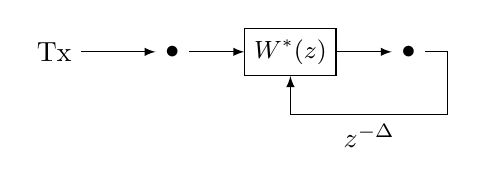
\begin{tikzpicture}[node distance=1.5cm, auto, >=latex]
    \node (tx) {Tx};
    \node [right of=tx] (dot1) {$\bullet$};
    \node [right of=dot1, draw, rectangle, minimum height=0.6cm] (hz) {\small $W^*(z)$};
    \node [right of=hz] (dot2) {$\bullet$};
    
    \draw [->] (tx) -- (dot1);
    \draw [->] (dot1) -- (hz);
    \draw [->] (hz) -- (dot2);
    
    % Feedback loop drawing
    \draw [->] (dot2) -- ++(0.5,0) |- ++(0,-0.8) -| node[pos=0.25, below] {$z^{-\Delta}$} (hz);
\end{tikzpicture}
\end{center}

For the first antenna, we modify $W^*(z)$ so that it can transform the first channel response into a delay $z^{-\Delta}$; the other channel response will not be such that the same $W^*(z)$ will be able to enforce the same delay as a result (at least if the response is different, which is generally the case): we've already used the only degree of freedom we had by setting $\Delta$.

\begin{remark}
In the MIMO case, we have more degrees of freedom and that's why we generally have a solution, provided that $\mathbf{H}$ is full rank.
\end{remark}

% Riquadro Verde - Esempio 2.18
\vspace{1em}
\noindent\setlength{\fboxsep}{10pt}\setlength{\fboxrule}{0.5pt}
\fcolorbox{teal}{teal!5}{%
    \parbox{\dimexpr\linewidth-2\fboxsep-2\fboxrule}{%
        \textbf{\textcolor{teal}{\faIcon{calculator} Example 2.18}}
        \vspace{0.5em}
        
        \textit{Compute the ZF equalizer for a frequency-flat channel with $N_r \geq N_t$.}
        \vspace{0.5em}
        
        In a frequency flat channel we can see that the matrix is just a pseudo inverse of $\mathbf{H}$, since we have $T = \mathbf{H} \rightarrow \text{delay of } L$.
        Then do not $L_{eq} \to \infty$ (minimize eq. error).
        
        We'll thus have:
        \begin{align}
            W^{ZF} = \frac{1}{\sqrt{C}} \mathbf{H}^+
        \end{align}
    }%
}
\vspace{1em}

There's a difference between the SISO and the MIMO cases.
\begin{itemize}
    \item \textbf{SISO:} we have the \textbf{problem of stability} and even for simple channels we might \textbf{not have a causal filter}.
    \item \textbf{MIMO:} The \textbf{perfect equalizer} of a \textbf{FIR channel is FIR}.
\end{itemize}

% Riquadro Blu/Viola - Esempio 2.19
\vspace{1em}
\noindent\setlength{\fboxsep}{10pt}\setlength{\fboxrule}{0.5pt}
\fcolorbox{blue}{blue!5}{%
    \parbox{\dimexpr\linewidth-2\fboxsep-2\fboxrule}{%
        \textbf{\textcolor{blue}{\faIcon{check-circle} Example 2.19}}
        \vspace{0.5em}
        
        \textit{Verify that the $W^{ZF}$ derived in Example 2.18 effects perfect ZF equalization.}
        \vspace{0.5em}
        
        \textbf{Solution}
        
        The application of the equalizer to the channel gives:
        \begin{align}
            W^{ZF}\sqrt{C}\mathbf{H} = (\mathbf{H}\mathbf{H}^+)^{-1}\mathbf{H}^H \mathbf{H} \implies \mathbf{I} \quad \text{Identity}
        \end{align}
        
        \textbf{If we ignore the noise, we have that the channel behaves like an Identity.}
    }%
}
\vspace{1em}

If we have 4 antennas in transmission and reception, it's like if we had 4 parallel channels: this is a big step forward.

\section{LMMSE equalization}

\begin{center}
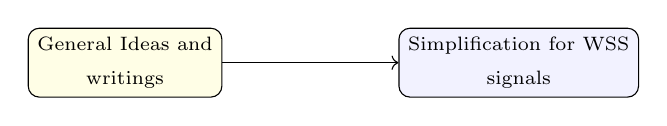
\begin{tikzpicture}
    \node[draw, fill=yellow!10, rounded corners, align=center] (a) {\scriptsize General Ideas and\\ \scriptsize writings};
    \node[draw, fill=blue!5, rounded corners, align=center, right of=a, node distance=5cm] (b) {\scriptsize Simplification for WSS\\ \scriptsize signals};
    \draw[->] (a) -- (b);
\end{tikzpicture}
\end{center}

Until now \textbf{we ignored noise}: the big problem with zero forcing which does not disappear with MIMO is that \textbf{noise generally gets amplified}.

If we multiply the $w$ with $y$, we get an error on top of the delay. We'll introduce a new concept, aka \textbf{trying to minimize the noise}. We're not just inverting the channel: we now have another target; we're trying to invert the channel as much as we can while also limiting the noise as much as we can.

ZF equalization neglects the noise: we instead would like to \textbf{take the noise into account}; in order to do so, we use the MMSE metric we already introduced. Our equalizer will then be a MMSE estimator and since we stay in the context of linear equalization, it will be a Linear MMSE estimator (LMMSE).

In this section we'll try to derive a LMMSE estimator using the theoretical concept we defined for MMSE estimation.

For this derivation we consider both $\mathbf{x}[n], \mathbf{s}[n]$ as \textbf{wide sense stationary}, using the notations:
\begin{align}
    R_x[l] &= E[\mathbf{x}[n]\mathbf{x}^*[n+l]] \\
    R_x[l] &= N_0 \delta[l] \cdot I
\end{align}
\textit{\footnotesize (Pass on this / get to some)}

\textit{\textcolor{green}{It can be shown}} that thanks to the transmit-receive relationships we defined:
\begin{align}
    R_y[l] &= G \sum_{i=0}^{L} \sum_{j=0}^{L} \mathbf{H}[i] R_x[l+i-j] \mathbf{H}^*[j] + N_0 \delta[l] I \label{eq:2.154} \\
    R_{yx}[l] &= \sqrt{G} \sum_{i=0}^{L} \mathbf{H}[i] R_x[l+i] \label{eq:2.158}
\end{align}

We want to look at the difference between $\mathbf{x}[n-\Delta]$ (which is the desired signal) and the equalized output (obtained by convolving the output $y$ ($N_r \times 1$) and the equalizer $W$ ($N_t \times N_r$)). We need to remember that $y$ will have the noise in it:
\begin{align}
    \hat{x}[n] - x[n - \Delta] = \sum_{l=0}^{L_{eq}} \mathbf{W}^*[l] \mathbf{y}[n-l] \label{eq:2.159}
\end{align}

% Riquadro Viola - Totally not trivial implication
\vspace{1em}
\noindent\setlength{\fboxsep}{10pt}\setlength{\fboxrule}{0.5pt}
\fcolorbox{violet}{violet!5}{%
    \parbox{\dimexpr\linewidth-2\fboxsep-2\fboxrule}{%
        \textbf{\textcolor{violet}{\faIcon{exclamation-triangle} Totally not trivial implication}}
        \vspace{0.5em}
        
        Differently from what we have in the original treatment, here we're not considering a frequency-flat channel. Rather, this channel has time dependency: for this reason, we're considering the convolution between $\mathbf{W}$ and $y$.
    }%
}
\vspace{1em}

\textbf{We want to minimize this difference here!} We can also obtain a matricial notation by stacking the various vectors/matrices; we'll obtain:
\begin{align}
    \mathbf{\hat{x}} = x[n-\Delta] - \mathbf{W}^* \vec{y}[n]
\end{align}

This is good to find the LMMSE estimator (\textit{in the book are all the details, professor does not really care about them}).

\begin{remark}
The book never states this explicitly, but those matrices are:
\begin{itemize}
    \item $W^* : N_t \times N_r (L_{eq} + 1)$
    \item $y[n] : N_r (L_{eq} + 1)$
\end{itemize}
And they're obtained through a simple stacking.
\end{remark}

Although neither the book or professor were really clear about this, I'd say that our equalizer is designed so that
\begin{align}
    \mathbf{W}^* y[n] \approx x[n-\Delta]
\end{align}
The problem is that ZF equalizers amplify the noise; we'd like to have a compromise between equalization of the channel and non-amplification of the noise.

We thus form the $W^{MMSE}$ estimator following from
\textbf{The estimator is simply}
\begin{align}
    \mathbf{W}^{LMMSE} = \mathbf{R}_y^{-1} \mathbf{R}_{yx} \label{eq:1.224}
\end{align}
which in this case (that of \textit{\textcolor{green}{WSS signals/noise}}) yields
\begin{align}
    W^{MMSE} &= \mathbf{R}_{\vec{y}[n]}^{-1} \mathbf{R}_{\vec{y}[n]x[n-\Delta]} \label{eq:3.102} \\
    &= \begin{bmatrix}
        R_y[0] & R_y[1] & \dots & R_y[L_{eq}] \\
        R_y[1] & R_y[0] & \dots & R_y[L_{eq}-1] \\
        \vdots & \vdots & \ddots & \vdots \\
        R_y[L_{eq}] & R_y[L_{eq}-1] & \dots & R_y[0]
    \end{bmatrix}^{-1}
    \begin{bmatrix}
        R_{yx}[-\Delta] \\
        R_{yx}[1-\Delta] \\
        \vdots \\
        R_{yx}[L_{eq}-\Delta]
    \end{bmatrix} \label{eq:2.163}
\end{align}

We then have that from
\begin{align}
    E &= \mathbb{E}[(\mathbf{x}-\hat{x})\mathbf{y}^H(\mathbf{x}-\hat{x})^H] \label{eq:1.241} \\
    &= \mathbf{R}_x - \mathbf{R}_{yx} - \mathbf{R}_{yx}^H + \mathbf{R}_y \label{eq:1.242} \\
    &= \mathbf{R}_x - \mathbf{W}^H \mathbf{R}_y^{-1} \mathbf{R}_{yx} - \dots \label{eq:1.243}
\end{align}
we can find the MMSE matrix by considering the various matrices we've already found, which will specifically give:
\begin{align}
    E &= \mathbb{E}[\tilde{x}[n]\tilde{x}^*[n]] \label{eq:2.164} \\
    &= R_x[0] - R_{yx[n]y[n]}^H R_{y[n]}^{-1} R_{yx[n]x[n-\Delta]} \label{eq:2.165}
\end{align}
% --- INIZIO CONTENUTO PAGINA ---

% Box Verde Chiaro - Nota Iniziale
\noindent\setlength{\fboxsep}{10pt}\setlength{\fboxrule}{0.5pt}
\fcolorbox{teal}{teal!5}{%
    \parbox{\dimexpr\linewidth-2\fboxsep-2\fboxrule}{%
        We don't need to remember the manipulations which are involved.\\
        There won't be exercises about this!
    }%
}
\vspace{1em}

% Box Rosso - Exam
\noindent\setlength{\fboxsep}{10pt}\setlength{\fboxrule}{0.5pt}
\fcolorbox{red}{red!5}{%
    \parbox{\dimexpr\linewidth-2\fboxsep-2\fboxrule}{%
        \textbf{\textcolor{red}{\faIcon{exclamation-circle} Exam}}
        \vspace{0.5em}
        
        We can bring 1A4 paper, with printings on only one side. We'll be able to use them for everything but not for the quizzes!!
    }%
}
\vspace{1em}

% Box Arancione - Warning
\noindent\setlength{\fboxsep}{10pt}\setlength{\fboxrule}{0.5pt}
\fcolorbox{orange}{orange!5}{%
    \parbox{\dimexpr\linewidth-2\fboxsep-2\fboxrule}{%
        \textbf{\textcolor{orange}{\faIcon{exclamation-triangle} Warning}}
        \vspace{0.5em}
        
        NEVER forget the noise, since it's the most important thing here.
    }%
}
\vspace{2em}

% Diagramma di flusso (riprodotto simile a quello precedente)
\begin{center}
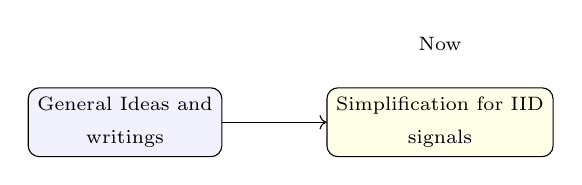
\begin{tikzpicture}[node distance=4cm, auto]
    \node[draw, fill=blue!5, rounded corners, align=center] (gen) {\scriptsize General Ideas and\\ \scriptsize writings};
    \node[draw, fill=yellow!10, rounded corners, align=center, right of=gen] (sim) {\scriptsize Simplification for IID\\ \scriptsize signals};
    \node[above of=sim, node distance=1cm] (now) {\scriptsize Now};
    
    \draw[->] (gen) -- (sim);
\end{tikzpicture}
\end{center}

If, in order to simplify things, we write as follows:

% Diagramma manuale "Ch coding -> S/P"
\begin{center}
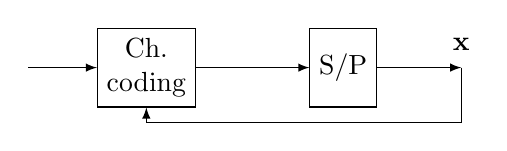
\begin{tikzpicture}[auto, >=latex]
    \node [draw, rectangle, minimum height=1cm, align=center] (ch) {Ch.\\ coding};
    \node [draw, rectangle, minimum height=1cm, right of=ch, node distance=2.5cm] (sp) {S/P};
    \node [coordinate, right of=sp, node distance=1.5cm] (end) {};
    \node [above of=end, node distance=0.3cm] (x) {$\mathbf{x}$};

    \draw [->] (-1.5,0) -- (ch);
    \draw [->] (ch) -- (sp);
    \draw [->] (sp) -- (end);
    
    % Feedback loop visivo abbozzato nel disegno originale
    \draw [->] (end) -- ++(0, -0.7) -| (ch);
\end{tikzpicture}
\end{center}

We have that the values of $\mathbf{x}$ are actually dependent, since the channel coding introduces dependencies and redundancy.

We make an \textbf{(incorrect!!)} assumption which is that the vector $\mathbf{x}$ is made of \textbf{IID symbols}; this assumption allows us to have a simple writing of $\mathbf{R}_x$:
\begin{align}
    R_x[l] = \frac{E_x}{N_t} \delta[l] I
\end{align}

If we choose $E_x$ in a specific manner, the $R_x$ matrix becomes an identity, which simplifies things by a lot.
This won't work in real systems, tho!

We'll obtain that the MMSE matrix can be written as:
\begin{align}
    \tilde{W}^{MMSE} &= \mathbf{R}_{\vec{y}[n]}^{-1} \mathbf{R}_{\vec{y}[n]x[n-\Delta]} \\
    &= \frac{1}{\sqrt{G}} \left( \mathcal{T}^H \mathcal{T} + \frac{N_t}{\text{SNR}} \mathbf{I} \right)^{-1} \mathcal{T}^H D \\
    &= \frac{1}{\sqrt{G}} \mathcal{T}^H \left( \mathcal{T} \mathcal{T}^H + \frac{N_t}{\text{SNR}} \mathbf{I} \right)^{-1} D
\end{align}

\textbf{The relevant thing is the SNR:} if we push the SNR to $+\infty$, we have that the noise is disappearing and we'll find again the zero forcing equalizer!
It makes sense that if the noise is disappearing the noise equalizer and the zero-forcing equalizer converge to be the same.

% Box Viola con Box Blu annidato
\vspace{1em}
\noindent\setlength{\fboxsep}{10pt}\setlength{\fboxrule}{0.5pt}
\fcolorbox{violet}{violet!5}{%
    \parbox{\dimexpr\linewidth-2\fboxsep-2\fboxrule}{%
        \textbf{\textcolor{violet}{\faIcon{sticky-note} This will never be asked, but for completeness:}}
        \vspace{0.5em}
        
        The $\mathcal{T}$ matrix is
        
        % Box Blu annidato (Toeplitz)
        \vspace{0.5em}
        \noindent\fcolorbox{blue}{white}{%
            \parbox{\dimexpr\linewidth-15pt}{%
                \textbf{\textcolor{blue}{\faIcon{pen} Toeplitz matrix $\mathcal{T}$}}
                \vspace{0.5em}
                
                The Toeplitz matrix $\mathcal{T}$ is defined as
                \begin{align}
                    \mathcal{T} = \begin{bmatrix}
                        H[0] & \dots & H[L] & 0 & \dots & 0 \\
                        0 & H[0] & \dots & H[L] & \dots & 0 \\
                        \vdots & & \ddots & & \ddots & \vdots \\
                        0 & \dots & 0 & H[0] & \dots & H[L]
                    \end{bmatrix} \label{eq:2.136}
                \end{align}
                having dimensions of $N_r(L_{eq}+1) \times N_t(L_{eq}+L+1)$.
            }%
        }
        \vspace{0.5em}
        
        and $D$ is all zeros except for
        \begin{align}
            [D]_{\Delta N_t : \Delta N_t + N_t - 1, :} = \mathbf{I}
        \end{align}
    }%
}
\vspace{1em}

The alternative form is obtained using the \textbf{\textcolor{green}{Matrix inversion lemma}}.
We know that this is a tool which is very much used.

What's important now is \textbf{the error}, which will be:
\begin{align}
    E = \frac{E_x}{N_t} \mathbf{I} - \frac{E_x}{N_t} D^T \mathcal{T}^* \left( \mathcal{T}\mathcal{T}^* + \frac{N_t}{\text{SNR}} \mathbf{I} \right)^{-1} \mathcal{T} D \label{eq:2.176}
\end{align}

\begin{quote}
    \textbf{\textcolor{red}{\small \faIcon{pen-fancy} Note:}}
    \textit{\textcolor{red}{EXAM TYPE OF QUESTION: demonstrate that G goes to zero if nr goes to infty}}
\end{quote}

If we \textbf{push the SNR to infinity}, we again have that the whole second term becomes $(E_x/N_t)I$ and thus we'd have $E \to 0$: we're again in the zero-forcing situation.

% Box Verde Chiaro - Errore
\vspace{1em}
\noindent\setlength{\fboxsep}{10pt}\setlength{\fboxrule}{0.5pt}
\fcolorbox{teal}{teal!5}{%
    \parbox{\dimexpr\linewidth-2\fboxsep-2\fboxrule}{%
        We didn't calculate the error in case of zero forcing; we'll see that the error is actually worse than this one.
    }%
}
\vspace{1em}

% Box Blu - Matrix of Matrices
\noindent\setlength{\fboxsep}{10pt}\setlength{\fboxrule}{0.5pt}
\fcolorbox{blue}{blue!5}{%
    \parbox{\dimexpr\linewidth-2\fboxsep-2\fboxrule}{%
        \textbf{\textcolor{blue}{\faIcon{pen} About the inversion of a matrix of matrices}}
        \vspace{0.5em}
        
        We can correctly invert a matrix by finding its determinant:
        \begin{align}
            A = \begin{bmatrix}
                d_{11} & d_{12} \\
                d_{21} & d_{22}
            \end{bmatrix}
        \end{align}
        \begin{align}
            \det(A) = d_{11}d_{22} - d_{12}d_{21}
        \end{align}
        
        \textit{Instead:}
        \begin{align}
            \mathcal{A} = \begin{bmatrix}
                A_{11} & A_{12} \\
                A_{21} & A_{22}
            \end{bmatrix}
        \end{align}
        
        We'll have
        \begin{align}
            \det(\mathcal{A}) = \det A_{11} \det A_{22} \\
             - \det A_{12} \det A_{21}
        \end{align}
        
        \vspace{0.5em}
        \hrule
        \vspace{0.5em}
        \footnotesize We can find this as reference 125 in the book.
    }%
}
\vspace{1em}

% Box Rosso - Recommended read
\noindent\setlength{\fboxsep}{10pt}\setlength{\fboxrule}{0.5pt}
\fcolorbox{red}{red!5}{%
    \parbox{\dimexpr\linewidth-2\fboxsep-2\fboxrule}{%
        \textbf{\textcolor{red}{\faIcon{times} Recommended read: example 2.21}}
        \vspace{0.5em}
        
        Example 2.21, which was mentioned by professor many times, uses (2.163) together with some other smart tricks in order to obtain the LMMSE estimator for frequency flat channels, using the precoding writing of the signal,
        \begin{align}
            x[n] - \sqrt{\frac{E_s}{N_t}} F[s] s[n] \label{eq:2.166}
        \end{align}
        , also assuming that the $s[n]$ symbols are IID, strict-sense stationary and unit-variance: this, together with the imposition that $\Delta = 0$, allows us to write that
        \begin{align*}
            \mathbf{R}_x[0] = \frac{E_s}{N_t}\mathbb{E}[\mathbf{F}[n]\mathbf{s}[n]\mathbf{s}^*[n]\mathbf{F}^*[n]] = \frac{E_s}{N_t}\mathbf{F}[n]\mathbf{F}^*[n]
        \end{align*}
        (which is admittedly a bit of a stretch, since the book just said that $\mathbf{R}_x[0] = \mathbf{F}\mathbf{F}^*$, assuming that all symbols are precoded through the same precoder and that $[0]$ expresses a delay of 0).

        In turn, this eventually allows us to write
        \begin{align}
            \mathbf{W}^{\text{MMSE}} = \frac{1}{\sqrt{G}} \left( \mathbf{H}\mathbf{F}\mathbf{F}^*\mathbf{H}^* + \frac{N_t}{\text{SNR}}\mathbf{I} \right)^{-1} \mathbf{H}\mathbf{F}, \tag{2.182}
        \end{align}
        for which we then have
    }%
}

% Box Rosso - Normally Asked Question (MIMO Eq)
\noindent\setlength{\fboxsep}{10pt}\setlength{\fboxrule}{0.5pt}
\fcolorbox{red}{red!5}{%
    \parbox{\dimexpr\linewidth-2\fboxsep-2\fboxrule}{%
        \textbf{\textcolor{red}{\faIcon{question-circle} Normally asked question: MIMO Eq}}
        \vspace{1em}

        \begin{center}
            
\includegraphics[width=0.6\textwidth]{Pictures/image.png}
        \end{center}
        
        \vspace{0.5em}
        
        \begin{minipage}[t]{0.6\textwidth}
            \textbf{What is the length of the equalizer?}
            \vspace{0.5em}
            
            $L_{eq} = 2$? $1$? \textbf{No.}
            \vspace{0.5em}
            
            $L_{eq}$ is \textbf{zero} because we don't have memory.
            \textbf{We have only a matrix.}
        \end{minipage}%
        \hfill
        \begin{minipage}[t]{0.35\textwidth}
            \centering
            \small
            \textit{Convention:}
            \begin{align*}
               \text{indices: } & \boxed{0}, 1, \dots, L_{eq} \\
               & \underbrace{\hspace{4em}}_{L_{eq} + 1}
            \end{align*}
        \end{minipage}
    }%
}
\vspace{1em}

% --- FINE CONTENUTO PAGINA ---
\end{document}

